\section{Governments' Regime Choice with Participation Asymmetry}

This section characterizes the governments' equilibrium standardization choices in stages 1--3, taking the stage-4 firm equilibria derived above as given. The key extension relative to the benchmark is that country $C$ may remain a weak participant in a common standard even after formal accession, because its post-investment residual compliance cost $\tau_C$ may remain high.

\subsection{Continuation welfare}

Because capacity investment is chosen at stage 0, the investment cost is sunk when governments choose among $SW$, $SU$, and $IS$ in stages 1--3. It is therefore convenient to define continuation welfare as
\begin{equation}
\widehat W_k^r \equiv CS_k^r + \pi_k^r,
\qquad r\in\{SW,SU,IS\},
\label{eq:cont_welfare_main}
\end{equation}
so that full national welfare is
\[
W_k^r=\widehat W_k^r-\frac{\eta}{2}I_k^2.
\]
Since the sunk investment term does not affect regime choice at stages 1--3, all continuation comparisons can be conducted using $\widehat W_k^r$.

By \eqref{eq:consumer_surplus}, consumer surplus in country $k$ under regime $r$ is
\begin{equation}
CS_k^r=\frac{(Q_k^r)^2}{2},
\label{eq:cs_main}
\end{equation}
where $Q_k^r$ is total quantity sold in market $k$ under regime $r$.

By symmetry, it is sufficient to consider country $A$ as the representative high-capacity member country and country $C$ as the lower-capacity outsider. Using \eqref{eq:QAsw_main}--\eqref{eq:QCis_main} together with \eqref{eq:piA_sw_main}--\eqref{eq:piC_is_main}, the continuation payoffs are
\begin{align}
\widehat W_A^r &= \frac{(Q_A^r)^2}{2}+\pi_A^r, \label{eq:WA_r_main}\\
\widehat W_C^r &= \frac{(Q_C^r)^2}{2}+\pi_C^r. \label{eq:WC_r_main}
\end{align}
The associated continuation world welfare is
\begin{equation}
\widehat W^r \equiv 2\widehat W_A^r+\widehat W_C^r.
\label{eq:world_continuation}
\end{equation}
Because stage-0 investment costs are sunk and common across regimes once
$(I_H,I_C)$ is fixed, ranking regimes by $\widehat W^r$ is equivalent to
ranking them by full world welfare. The explicit closed forms are reported in
Appendix~A.

\subsection{Welfare differences}

The stagewise regime choice is governed by four continuation-welfare differences:
\begin{align}
\Delta_A^I
&\equiv
\widehat W_A^{IS}-\widehat W_A^{SU}, \label{eq:DeltaAI_main}\\
\Delta_C^I
&\equiv
\widehat W_C^{IS}-\widehat W_C^{SU}, \label{eq:DeltaCI_main}\\
\Delta_A^{SU}
&\equiv
\widehat W_A^{SU}-\widehat W_A^{SW}, \label{eq:DeltaASU_main}\\
\Delta_A^{IS}
&\equiv
\widehat W_A^{IS}-\widehat W_A^{SW}. \label{eq:DeltaAIS_main}
\end{align}

On the admissible parameter set $\mathcal P$, all denominators in these differences are strictly positive. Hence their signs are fully characterized by the numerator polynomials reported in Appendix~A. This allows the equilibrium regime to be described directly in terms of the signs of \eqref{eq:DeltaAI_main}--\eqref{eq:DeltaAIS_main}.

\subsection{Stage 3: acceptance of country \texorpdfstring{$C$}{C}}

Suppose that countries $A$ and $B$ have already formed a two-country standardization union and that country $C$ requests accession. Since $A$ and $B$ are symmetric, both member governments accept country $C$ if and only if a representative member country weakly prefers full international standardization to retaining the two-country bloc:
\begin{equation}
\Delta_A^I \ge 0.
\label{eq:accept_rule_main}
\end{equation}

Condition \eqref{eq:accept_rule_main} summarizes the member countries' trade-off. Moving from $SU$ to $IS$ enlarges the installed base and reduces cross-border friction for country $C$, but it also intensifies competition in member-country markets. When country $C$'s participation capacity is sufficiently low, the added network benefit from accession is small relative to the additional competitive pressure, and the incumbent members reject accession.

\subsection{Stage 2: accession request by country \texorpdfstring{$C$}{C}}

Conditional on a two-country union having been formed, country $C$ requests accession if and only if it weakly prefers full international standardization to remaining excluded from the bloc:
\begin{equation}
\Delta_C^I \ge 0.
\label{eq:join_rule_main}
\end{equation}

Thus, accession to the common standard requires two separate inequalities: country $C$ must want to join, and the incumbent member countries must be willing to admit it. This distinction is immaterial in models where accession removes all relevant frictions, but it is central here because formal membership and effective participation need not coincide.

\subsection{Stage 1: formation of a two-country union}

At stage 1, countries $A$ and $B$ decide whether to initiate bilateral harmonization, anticipating the continuation path in stages 2 and 3.

If both
\begin{equation}
\Delta_C^I \ge 0
\qquad\text{and}\qquad
\Delta_A^I \ge 0,
\label{eq:is_path_main}
\end{equation}
hold, then country $C$ requests accession and countries $A$ and $B$ accept it. In that case, initiating bilateral harmonization at stage 1 leads to full international standardization. Therefore, countries $A$ and $B$ form the initial union if and only if
\begin{equation}
\Delta_A^{IS} \ge 0.
\label{eq:form_is_main}
\end{equation}

If, by contrast,
\begin{equation}
\Delta_C^I < 0
\qquad\text{or}\qquad
\Delta_A^I < 0,
\label{eq:su_path_main}
\end{equation}
then the accession step fails, either because country $C$ does not apply or because the member countries reject its request. In that case, initiating bilateral harmonization leads only to a two-country standardization union, and countries $A$ and $B$ form it if and only if
\begin{equation}
\Delta_A^{SU} \ge 0.
\label{eq:form_su_main}
\end{equation}

Because the game is solved by backward induction, the relevant comparison at
stage 1 is the realized continuation payoff implied by the entire downstream
path, not the payoff from an $A$--$B$ union viewed in isolation. In
particular, when bloc formation at stage 1 leads to accession and hence to $IS$
at stage 3, the member-country comparison is with the $IS$ continuation payoff
rather than with the $SU$ continuation payoff alone.

\subsection{Equilibrium regime}

The preceding inequalities yield the following characterization.

\begin{proposition}[Equilibrium regime with participation-capacity asymmetry]
Fix post-investment capacities $(\tau,\tau_C)$ and suppose that $(v,c,\tau,\tau_C)\in\mathcal P$.

\begin{enumerate}
    \item The equilibrium regime is $IS$ if and only if
    \[
    \Delta_C^I \ge 0,\qquad
    \Delta_A^I \ge 0,\qquad
    \Delta_A^{IS} \ge 0.
    \]

    \item The equilibrium regime is $SU$ if and only if
    \[
    \bigl(\Delta_C^I<0 \ \text{or}\ \Delta_A^I<0\bigr)
    \quad\text{and}\quad
    \Delta_A^{SU}\ge 0.
    \]

    \item The equilibrium regime is $SW$ otherwise.
\end{enumerate}
\label{prop:regime_choice_main}
\end{proposition}

\begin{proof}
The argument is by backward induction. At stage 3, accession is accepted if and only if \eqref{eq:accept_rule_main} holds. At stage 2, country $C$ requests accession if and only if \eqref{eq:join_rule_main} holds. Hence, if both inequalities in \eqref{eq:is_path_main} are satisfied, initiating bilateral harmonization at stage 1 leads to $IS$, and the relevant comparison is \eqref{eq:form_is_main}. Otherwise, the accession path fails and initiating bilateral harmonization leads only to $SU$, so the relevant comparison is \eqref{eq:form_su_main}. The three cases in Proposition~\ref{prop:regime_choice_main} follow immediately and are exhaustive.
\end{proof}

Figure~\ref{fig:regime_map} provides a visual summary of the regime partition
characterized in Proposition~\ref{prop:regime_choice_main}.

\begin{figure}[t]
\centering
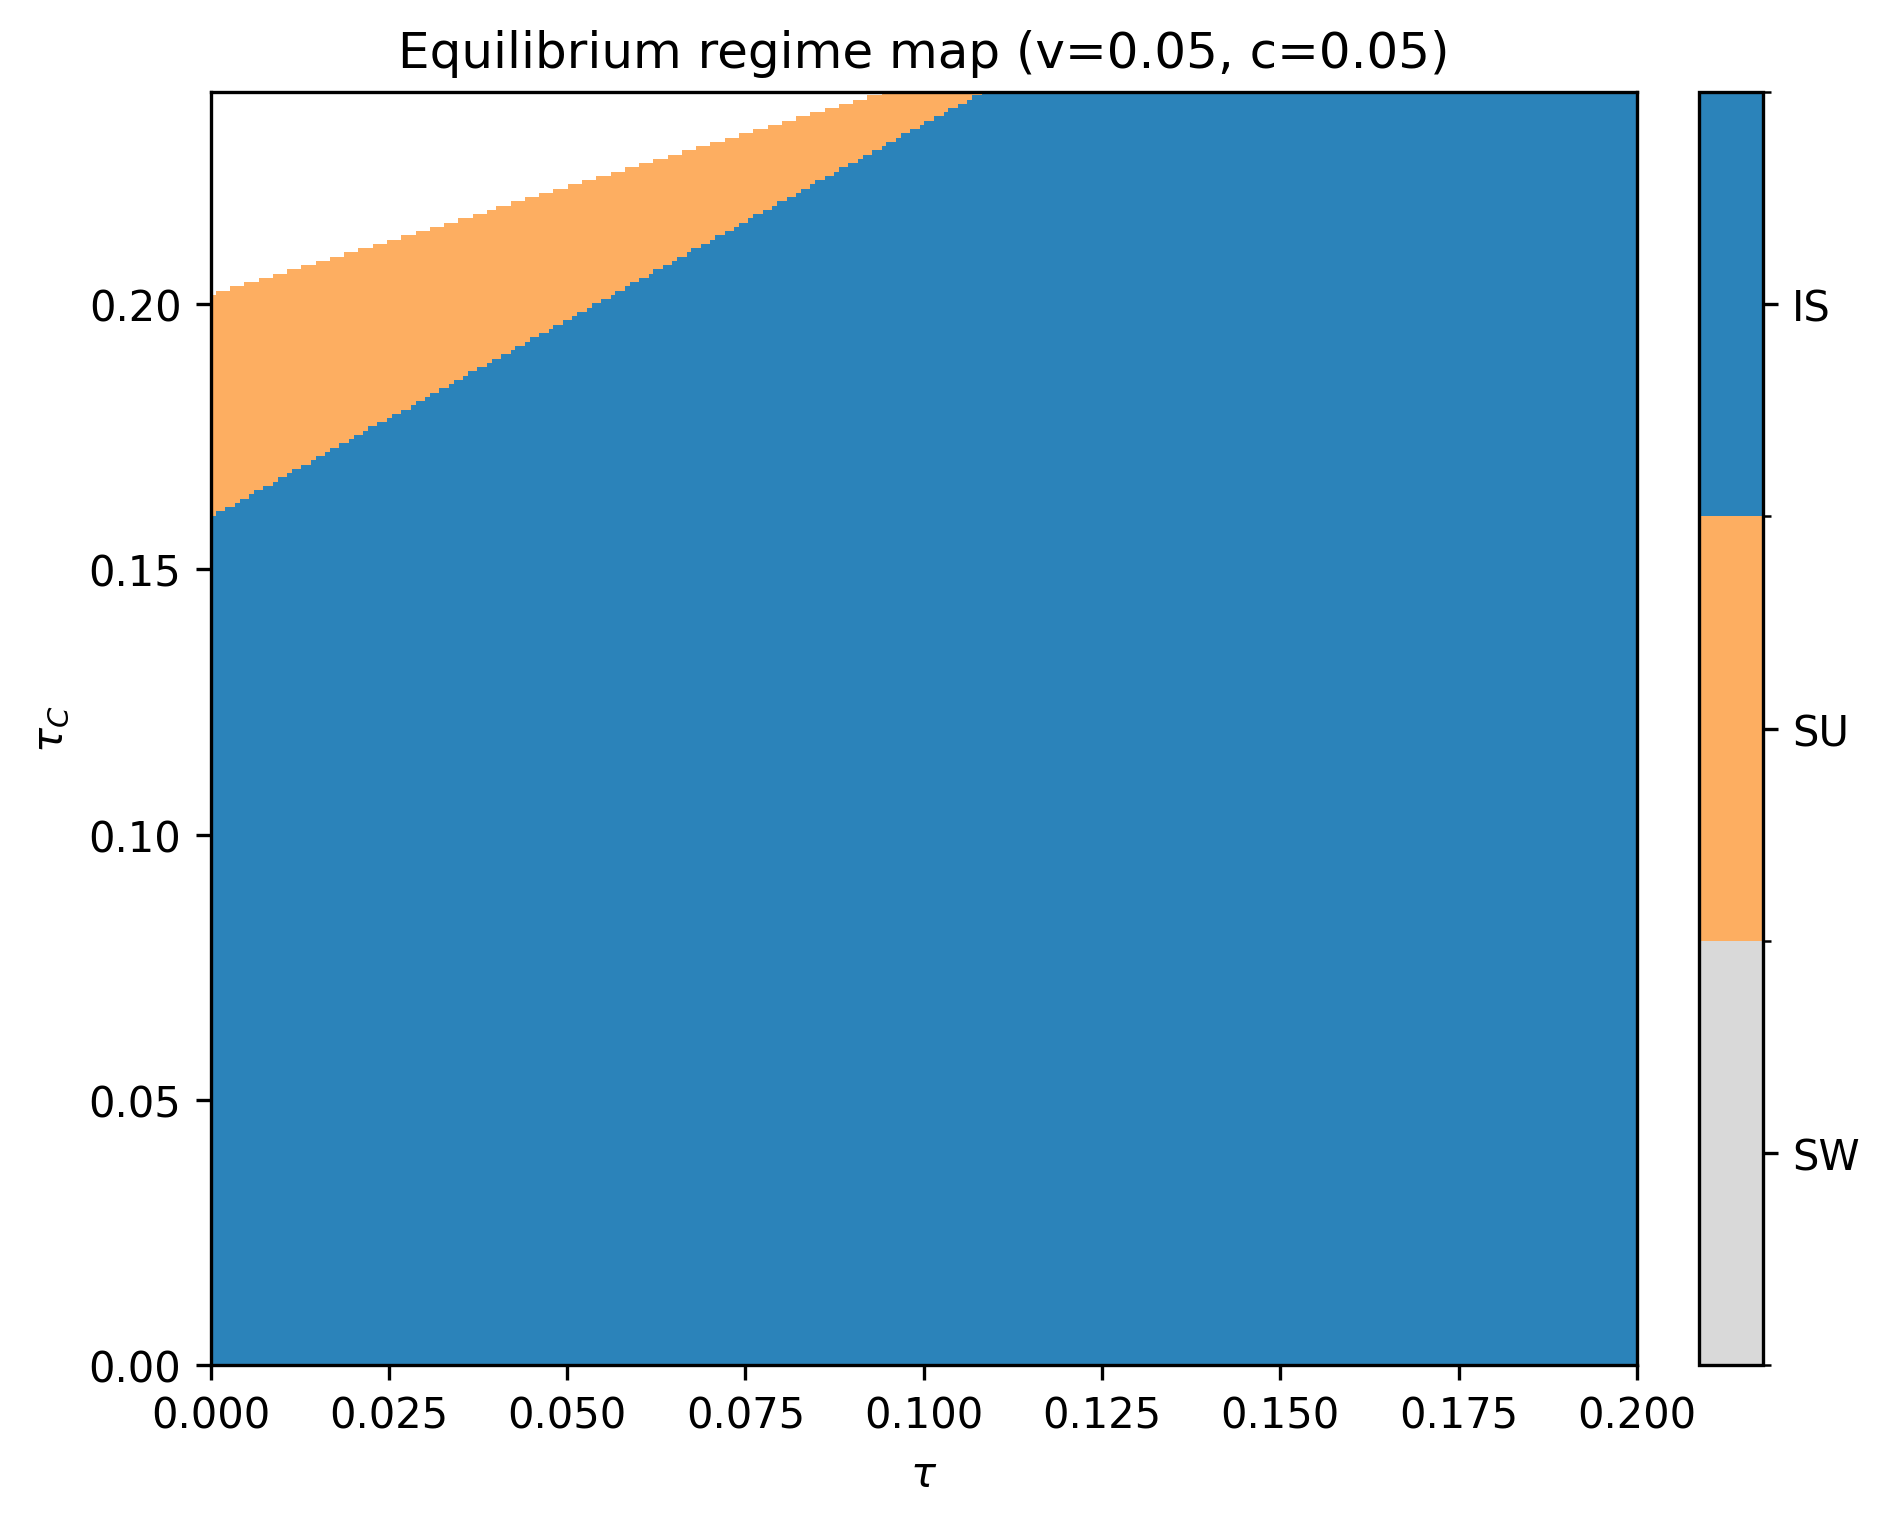
\includegraphics[width=.82\linewidth]{figures/fig2_regime_map.png}
\caption{Equilibrium regime map in $(\tau,\tau_C)$. For fixed $(v,c)$, the figure partitions the $(\tau,\tau_C)$ plane into the regions in which the equilibrium regime characterized by Proposition~\ref{prop:regime_choice_main} is $SW$, $SU$, or $IS$. The map illustrates how outsider-side participation frictions and member-country residual compliance costs jointly determine whether the equilibrium outcome is no harmonization, an exclusionary two-country bloc, or full international standardization.}
\label{fig:regime_map}
\end{figure}

\subsection{World welfare versus equilibrium regime}

The equilibrium characterization in Proposition~\ref{prop:regime_choice_main}
need not coincide with the continuation world-welfare ranking. The next
proposition states the divergence highlighted in the abstract and introduction.

\begin{proposition}[World welfare and equilibrium regime may diverge]
There exists a nonempty subset $\Omega\subset \mathcal P$ such that
\[
\widehat W^{IS}>\max\{\widehat W^{SU},\widehat W^{SW}\},
\]
while the equilibrium regime characterized in
Proposition~\ref{prop:regime_choice_main} is $SU$. Equivalently, for fixed
stage-0 investments, full international standardization can maximize world
welfare without arising in equilibrium.
\label{prop:welfare_gap_main}
\end{proposition}

\begin{proof}
Consider the parameter point
\[
(v,c,\tau,\tau_C)=(0.05,\,0.05,\,0.02,\,0.18).
\]
Using the closed-form continuation-welfare formulas from Appendix~A gives
\[
\widehat W^{SW}\approx 1.24426,\qquad
\widehat W^{SU}\approx 1.54410,\qquad
\widehat W^{IS}\approx 1.67046.
\]
Hence $IS$ strictly maximizes continuation world welfare at this point.
Meanwhile,
\[
\Delta_C^I\approx 0.12788>0,\qquad
\Delta_A^I\approx -0.00076<0,\qquad
\Delta_A^{SU}\approx 0.15189>0.
\]
By Proposition~\ref{prop:regime_choice_main}, the equilibrium regime is
therefore $SU$. Because all inequalities are strict and the closed-form
continuation payoffs are continuous on $\mathcal P$, there exists an open
neighborhood $\Omega$ of this point on which the same inequalities continue to
hold. This proves the claim.
\end{proof}

\noindent\textbf{A one-dimensional characterization of the divergence region.}
The numerical point used in Proposition~\ref{prop:welfare_gap_main} is not
isolated. Fix
\[
(v,c,\tau)=(0.05,0.05,0.02)
\]
and let $\tau_C$ vary. Along this line, the admissibility condition
$1-2c+\tau-3\tau_C>0$ implies
\[
\tau_C<\bar\tau_C^{\,adm}\equiv \frac{1-2c+\tau}{3}=0.306\overline{6}.
\]
Using the closed-form continuation payoffs, the incumbent-acceptance margin
$\Delta_A^I(\tau_C)$ crosses zero at
\[
\tau_C^\dagger \approx 0.1750504.
\]
Moreover, along the same line, both $\Delta_C^I(\tau_C)$ and
$\widehat W^{IS}(\tau_C)-\widehat W^{SU}(\tau_C)$ remain strictly positive
throughout the admissible interval, and $\Delta_A^{SU}(\tau_C)$ is also
strictly positive. Hence for every
\[
\tau_C\in(\tau_C^\dagger,\bar\tau_C^{\,adm}),
\]
the equilibrium regime is $SU$ while continuation world welfare is strictly
higher under $IS$. Thus, Proposition~\ref{prop:welfare_gap_main} is supported
not only by a single benchmark point, but by a nondegenerate interval of
outsider-side compliance costs.

Figure~\ref{fig:divergence_map} shows that the welfare-equilibrium divergence
identified in Proposition~\ref{prop:welfare_gap_main} is not a knife-edge
phenomenon.

\begin{figure}[t]
\centering
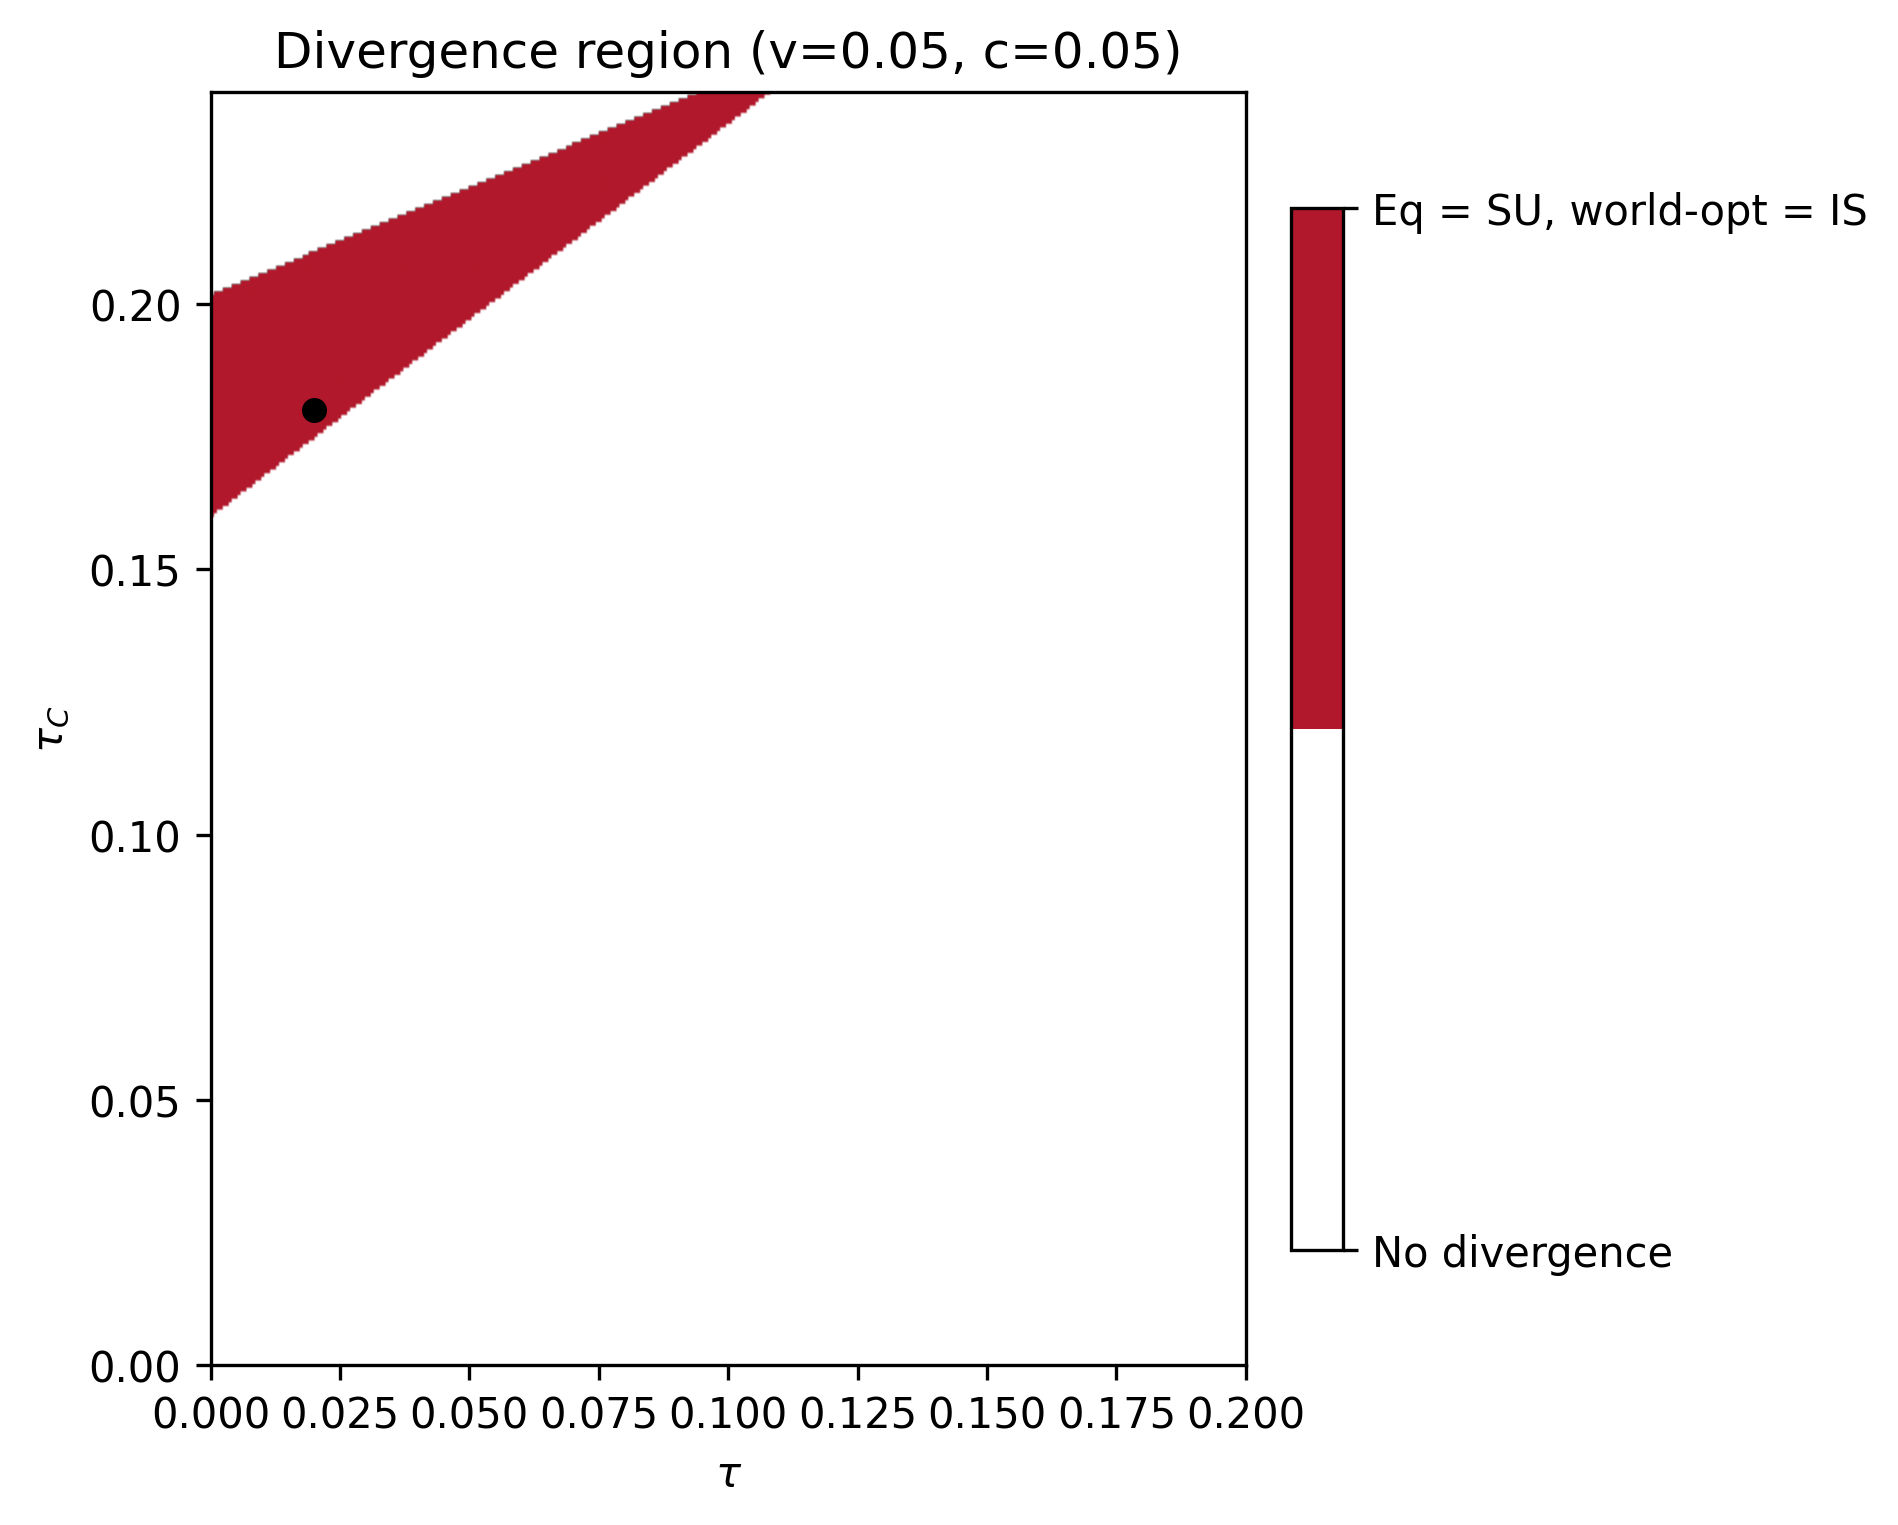
\includegraphics[width=.82\linewidth]{figures/fig3_divergence_map.png}
\caption{Region where the equilibrium regime is $SU$ but the world-optimal regime is $IS$. For fixed $(v,c)$, the shaded region identifies parameter combinations for which incumbent-country incentives sustain an exclusionary two-country bloc even though continuation world welfare is maximized by full international standardization. The benchmark point used in Proposition~\ref{prop:welfare_gap_main}, $(v,c,\tau,\tau_C)=(0.05,0.05,0.02,0.18)$, is marked for reference.}
\label{fig:divergence_map}
\end{figure}

\begin{proposition}[Stronger network effects can stabilize an exclusionary bloc]
There exist parameters $(c,\tau,\tau_C)$ and two network-effect values
$0\le v'<v''<2/7$ such that the equilibrium regime is $IS$ at
$(v',c,\tau,\tau_C)$ but $SU$ at $(v'',c,\tau,\tau_C)$. In particular,
stronger network effects need not favor full harmonization uniformly; they can
instead stabilize an exclusionary two-country standards bloc.
\label{prop:network_bloc_main}
\end{proposition}

\begin{proof}
Consider the common cost profile
\[
(c,\tau,\tau_C)=(0.05,\,0,\,0.15).
\]
At $v'=0.04$, the continuation-welfare differences are
\[
\Delta_A^I\approx 0.00424>0,\qquad
\Delta_C^I\approx 0.11303>0,\qquad
\Delta_A^{IS}\approx 0.12668>0.
\]
By Proposition~\ref{prop:regime_choice_main}, the equilibrium regime is
therefore $IS$.

At $v''=0.055$, the same cost profile yields
\[
\Delta_A^I\approx -0.00026<0,\qquad
\Delta_C^I\approx 0.15025>0,\qquad
\Delta_A^{SU}\approx 0.17261>0.
\]
Hence Proposition~\ref{prop:regime_choice_main} implies that the equilibrium
regime is $SU$. The inequalities are strict at both parameter points, so the
same regime rankings persist on open neighborhoods around them.
\end{proof}

\noindent\textbf{A one-dimensional threshold characterization for Proposition~\ref{prop:network_bloc_main}.}
The mechanism in Proposition~\ref{prop:network_bloc_main} can also be made
more explicit along a fixed cost profile. Set
\[
(c,\tau,\tau_C)=(0.05,0,0.15)
\]
and let $v$ vary. Along this line, the member-country accession margin
$\Delta_A^I(v)$ crosses zero at
\[
v^\dagger \approx 0.0543568.
\]
For $v<v^\dagger$, we have $\Delta_A^I(v)>0$, whereas for $v>v^\dagger$,
$\Delta_A^I(v)<0$. At the same time, $\Delta_C^I(v)>0$,
$\Delta_A^{SU}(v)>0$, and $\widehat W^{IS}(v)-\widehat W^{SU}(v)>0$ continue
to hold throughout the admissible interval in which $SU$ remains interior. In
particular, the relevant admissible upper bound along this line is
\[
\bar v^{\,adm}\approx 0.0756400.
\]
Hence for every
\[
v\in(v^\dagger,\bar v^{\,adm}),
\]
the equilibrium regime is $SU$ even though continuation world welfare remains
strictly higher under $IS$. This yields a one-dimensional threshold
characterization of the network-effect mechanism behind
Proposition~\ref{prop:network_bloc_main}.

\subsection{Interpretation}

Propositions~\ref{prop:regime_choice_main} and \ref{prop:welfare_gap_main}
highlight the role of participation-capacity asymmetry. Even when full
international standardization is technologically feasible, it may fail to arise
for two distinct reasons. First, country $C$ may not find accession attractive
if its residual compliance cost remains too high. Second, even if country $C$
wishes to join, incumbent member countries may reject accession because country
$C$ adds too little to the common network relative to the intensified
competition it creates in member-country markets.

The mechanism behind Proposition~\ref{prop:welfare_gap_main} is straightforward.
When country $C$ has low participation capacity, accession to the common
standard removes the baseline technology-gap cost but still leaves $C$ with a
relatively weak effective competitive position. From the perspective of member
countries $A$ and $B$, accession then delivers only a limited increase in the
common installed base, while it nevertheless introduces additional competition
in member-country markets. As a result, full international standardization can
raise world welfare and still fail the incumbent members' private acceptance
test.

The comparative statics in Appendix~B help sharpen this logic. On the verified
compact domain used in Section~5, both $\Delta_A^I$ and $\Delta_C^I$ decline as
$\tau_C$ rises. Intuitively, a larger outsider-side compliance burden weakens
the outsider's effective market participation even after formal accession. Yet
$\Delta_C^I$ may remain positive longer than $\Delta_A^I$, because country $C$
still values the removal of the baseline technology-gap cost under $IS$, while
member governments internalize the additional competition in their own markets.

Proposition~\ref{prop:network_bloc_main} shows that the network parameter $v$
does not operate monotonically in favor of full harmonization. Stronger network
effects magnify the installed-base gain from common recognition, but they also
raise the strategic value of preserving an incumbent bloc when outsider
participation remains weak. Accordingly, an exclusionary two-country standards
bloc may persist not only because incumbent countries strategically prefer
exclusion, but also because the outsider's participation capacity is too weak
for full harmonization to be privately attractive.
